% Section V: Results. Numbers (all under results/metrics/):
%   feature_check.csv (Fig. feature check), cv_check.csv (Table cvcheck),
%   cv_results.csv and final_model.json (CV errors, final model),
%   test_results.csv (Table test), error_breakdown.csv (Table breakdown),
%   floor_confusion.csv (Fig. confusion; 81 of the 87 wrong floors are one
%   floor off), per_phone.csv (seen and new phones, last paragraph).
\section{Results}\label{sec:results}

\begin{figure}[t]
  \centering
  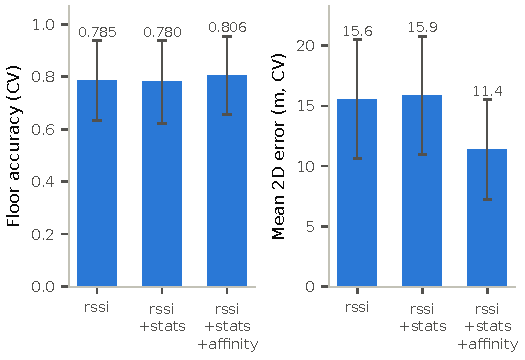
\includegraphics[width=0.95\columnwidth]{feature_check.pdf}
  \caption{Feature check: the Baseline RF settings on the three feature sets
  under user-group CV (bars: mean over the five folds; error bars: standard
  deviation). Floor accuracy is shown as a fraction.}
  \label{fig:features}
\end{figure}

\subsection{Feature Check}\label{sec:res-features}
Fig.~\ref{fig:features} shows the Baseline RF settings on the three feature
sets under user-group CV. The signal statistics did not help: the mean 2D error
rose slightly from 15.55 to 15.87~m and floor accuracy fell from 78.5\% to
78.0\%. AP-affinity helped clearly: the error fell to 11.38~m and floor accuracy
rose to 80.6\%. We keep the statistics in the full set because the three sets
are nested and the full set scored best; we did not test rssi plus AP-affinity
alone. The wide error bars show that the folds differ a lot, as each holds out
different people and places.

\begin{table}[t]
  \caption{The Baseline RF Scored in Three Ways}
  \label{tab:cvcheck}
  \centering
  \footnotesize
  \begin{tabular}{@{}lrrr@{}}
    \toprule
    Evaluation & Building (\%) & Floor (\%) & Mean 2D error (m) \\
    \midrule
    Random CV     & 100.0 & 99.9 &  3.67 \\
    User-group CV &  99.7 & 78.0 & 15.87 \\
    Test set      &  99.8 & 91.2 & 12.52 \\
    \bottomrule
  \end{tabular}
\end{table}

\subsection{Random CV Is Too Optimistic}\label{sec:res-cv}
For the same Baseline RF, random CV promised 99.9\% floor accuracy and a mean
2D error of 3.67~m, but the test set gave 91.2\% and 12.52~m
(Table~\ref{tab:cvcheck}): random CV tests the model on scans that look
almost like its training scans (same spot, person and phone). User-group CV
(15.87~m) is even stricter than the test set, as a held-out user may be the
only one who recorded some places. It errs on the safe side and needs no test data, so we
make all choices with it.

\begin{figure*}[t]
  \centering
  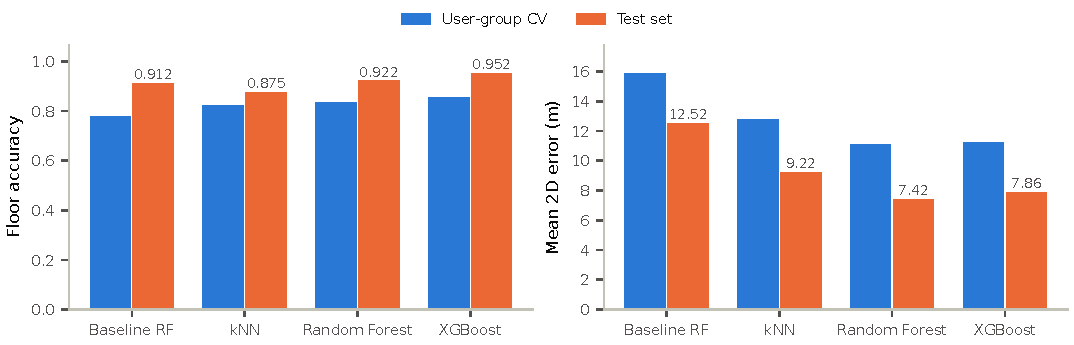
\includegraphics[width=0.9\textwidth]{model_comparison.pdf}
  \caption{Floor accuracy (as a fraction) and mean 2D error of the four models
  in user-group CV and on the test set (test values above the bars).}
  \label{fig:models}
\end{figure*}

\begin{table}[t]
  \caption{Results on the Test Set (1,111 Scans)}
  \label{tab:test}
  \centering
  \footnotesize
  \setlength{\tabcolsep}{3.5pt}
  \begin{tabular}{@{}lrrrrrr@{}}
    \toprule
    & Bldg. & Floor & MAE $x$ & MAE $y$ & \multicolumn{2}{c}{2D error (m)} \\
    \cmidrule(l){6-7}
    Model & (\%) & (\%) & (m) & (m) & Mean & Median \\
    \midrule
    Baseline RF   &  99.8 & 91.2 & 8.68 & 7.40 & 12.52 & 7.70 \\
    kNN           &  99.8 & 87.5 & 6.12 & 5.70 &  9.22 & 5.88 \\
    Random Forest & \textbf{100.0} & 92.2 & \textbf{4.77} & \textbf{4.64}
                  & \textbf{7.42} & \textbf{5.34} \\
    XGBoost       & \textbf{100.0} & \textbf{95.2} & 5.18 & 4.77 & 7.86 & 6.19 \\
    \bottomrule
  \end{tabular}
\end{table}

\subsection{Model Comparison}\label{sec:res-models}
Random Forest had the lowest CV mean 2D error (11.09~m, against 11.25~m for
XGBoost and 12.75~m for kNN), so by our rule it is the final model. On the test
set (Table~\ref{tab:test}) it found the building of every scan and the floor of
92.2\%, with a mean 2D error of 7.42~m, against 12.52~m for the Baseline RF.
The four models keep the same order by mean 2D error in CV and on the test set
(Fig.~\ref{fig:models}), so the choice made with CV holds. XGBoost, however,
found the most floors (95.2\% on the test set, 85.4\% in CV): no model is best
at every task.

\begin{table}[t]
  \caption{Where the Test Error Comes From}
  \label{tab:breakdown}
  \centering
  \footnotesize
  \setlength{\tabcolsep}{4pt}
  \begin{tabular}{@{}lrrr@{}}
    \toprule
    & Share of & Mean 2D & Share of total \\
    Case & scans (\%) & error (m) & error (\%) \\
    \midrule
    \multicolumn{4}{@{}l}{\emph{Random Forest}} \\
    Building wrong              &  0.0 &    -- &  0.0 \\
    Building right, floor wrong &  7.8 & 13.06 & 13.8 \\
    Both right                  & 92.2 &  6.94 & 86.2 \\
    \midrule
    \multicolumn{4}{@{}l}{\emph{XGBoost}} \\
    Building wrong              &  0.0 &    -- &  0.0 \\
    Building right, floor wrong &  4.8 & 14.78 &  9.0 \\
    Both right                  & 95.2 &  7.52 & 91.0 \\
    \bottomrule
  \end{tabular}
\end{table}

\begin{figure*}[t]
  \centering
  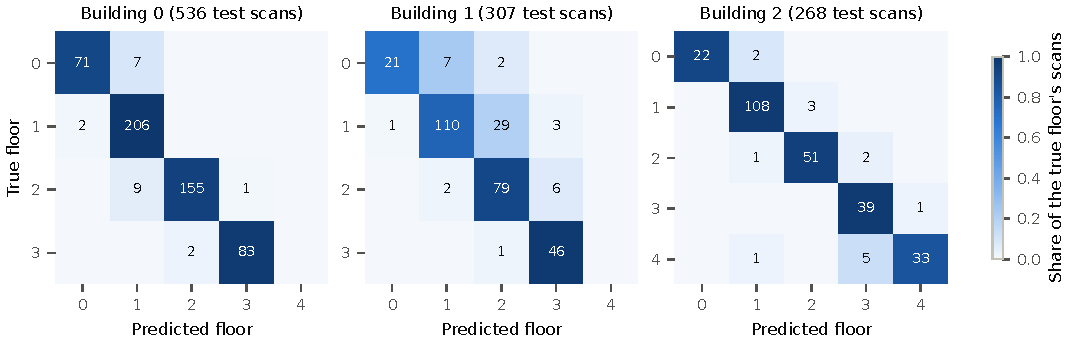
\includegraphics[width=0.95\textwidth]{floor_confusion.pdf}
  \caption{Floor confusion of the final model (Random Forest) on the test set:
  test scans per true and predicted floor; colors show the true floor's share.}
  \label{fig:confusion}
\end{figure*}

\subsection{Where the Error Comes From}\label{sec:res-errors}
Neither Random Forest nor XGBoost put a test scan in the wrong building; the
Baseline RF and kNN did so twice each. For the Random Forest, 87 scans (7.8\%) have the
right building but the wrong floor, and their mean 2D error (13.06~m) is nearly
twice that of the scans with both right (6.94~m; Table~\ref{tab:breakdown}).
Still, 86.2\% of the total error comes from the scans with both right: the main
remaining problem is the position within the right floor. Of the 87 floor
mistakes, 81 are one floor up or down (Fig.~\ref{fig:confusion}), and
building~1 has the most; for example, 29 of its floor-1 scans were placed on
floor~2. XGBoost makes fewer floor mistakes (53) but has a higher error when
both are right (7.52~m).

New phones are harder. On the 397 test scans from the 2 phones seen in
training, the Random Forest has a mean 2D error of 5.84~m and a floor accuracy
of 93.7\%; on the 714 scans from the 9 new phones, 8.30~m and 91.3\%. All four
models are worse on new phones.
